% !TeX root = er.tex

\chapter{Commande à logique floue}\label{ch.fuzzy}
\index{logique floue}

Les algorithmes de contrôle du chapitre \ref{ch.control} utilisaient des calculs mathématiques exacts pour déterminer les signaux utilisés pour contrôler le comportement d'un robot. Une autre approche consiste à utiliser des algorithmes de contrôle basés sur des \emph{règles}. Un système de régulation de vitesse pourrait avoir des règles de la forme suivante :
\begin{itemize}
\item Si la \emph{voiture de devant est loin} ou la \emph{voiture de derrière est proche}, réglez la \emph{vitesse sur rapide}.
\item Si la \emph{voiture de devant est proche}, réglez la \emph{vitesse sur lente}.
\end{itemize}
La logique est "floue" parce que les règles sont exprimées en termes de \emph{variables linguistiques} comme \emph{vitesse} dont les valeurs n'ont pas de définitions mathématiques précises, mais seulement des spécifications linguistiques imprécises comme \emph{rapide} et \emph{lente}.

Un contrôleur à logique floue se compose de trois phases qui s'exécutent de manière séquentielle :
\begin{description}
\item[\textbf{Flouter}] Les valeurs des capteurs sont converties en valeurs de variables linguistiques, telles que \p{loin}, \p{en approche}, \p{près}, appelées \emph{prémisses}. Chaque prémisse spécifie une \emph{probabilité} qui est la probabilité de notre conviction que la variable est vraie.
\item[\textbf{Appliquer les règles}] Un ensemble de \emph{règles} exprime l'algorithme de contrôle. Étant donné un ensemble de prémisses, une \emph{valeur} est déduite. Les valeurs sont également des variables linguistiques telles que \p{très rapide}, \p{rapide}, \p{vitesse de croisière}, \p{lent}, \p{arrêt}.
\item[\textbf{Déflouter}] Les valeurs sont combinées afin de produire une sortie \emph{pertinente}, une valeur numérique qui contrôle certains aspects du robot tels que la puissance appliquée aux moteurs.
\end{description}

Les sections suivantes présentent les trois phases du contrôle flou pour la tâche d'un robot s'approchant d'un objet et s'arrêtant lorsqu'il est très proche de l'objet.

\section{Flouter}

Lors de l'approche d'un objet, la valeur lue par le capteur de proximité horizontal passe de $0$ à $100$. La valeur renvoyée par le capteur est rendue floue en la convertissant en valeur d'une variable linguistique. La figure \ref{fig.fuzz} montre trois graphiques permettant de convertir les valeurs du capteur en probabilités des variables linguistiques \index{fuzzy logic!linguistic variable} \p{loin}, \p{en approche} et \p{près}. L'axe $x$ est la valeur renvoyée par le capteur et l'axe $y$ donne la prémisse pour chaque variable, la probabilité que la variable linguistique est vraie.


\begin{figure}
\begin{center}
% Fuzzify a horizontal proximity sensor
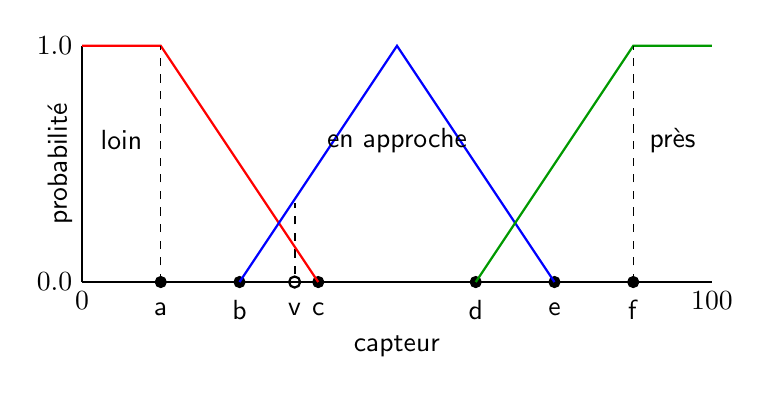
\begin{tikzpicture}
\draw (0,0) node[left] {\p{0.0}} node[below] {\p{0}} -- node[sloped,above] {\textsf{probabilité}} (0,3) node[left] {\p{1.0}};
\draw (0,0) -- node[below,yshift=-16pt] {\textsf{capteur}} (8,0) node[below] {\p{100}};
\foreach \n/\x in {a/1,b/2,c/3,d/5,e/6,f/7} {
  \draw[fill] (\x,0) circle [radius=2pt];
  \node at (\x,-10pt) { \textsf{\n} };
}
\draw[thick] (2.7,0) circle [radius=2pt];
\node at (2.7,-10pt) { \textsf{v} };
\draw[dashed,thick] (2.7,.1) -- +(0,.9);
\draw[red,thick] (0,3) -- (1,3) -- (3,0);
\draw[blue,thick] (2,0) -- (4,3) -- (6,0);
\draw[green!60!black,thick] (5,0) -- (7,3) -- (8,3);
\draw[dashed] (1,0) -- (1,3);
\draw[dashed] (7,0) -- (7,3);
\node at (.5,1.8) {\textsf{loin}};
\node at (4,1.8) {\textsf{en approche}};
\node at (7.5,1.8) {\textsf{près}};
\end{tikzpicture}
\caption{Flouter la valeur du capteur de proximité horizontal}\label{fig.fuzz}
\end{center}
\end{figure}

Les points étiquetés sur l'axe $x$ correspondent aux seuils : (a) \p{far\_low}, (b) \p{closing\_low}, (c) \p{far\_high}, (d) \p{near\_low}, (e) \p{closing\_high}, (f) \p{near\_high}. Si la valeur du capteur est inférieure à \p{far\_low}, nous sommes totalement certains que l'objet est éloigné et la probabilité est de $1$. Si la valeur est comprise entre \p{closing\_low} et \p{far\_high}, nous sommes quelque peu certains que l'objet est éloigné, mais aussi quelque peu certains qu'il se rapproche. Le flou résulte du chevauchement des plages : lorsque la valeur se situe entre le point (b) et le point (c), nous ne pouvons pas dire avec une probabilité absolue si l'objet est éloigné ou s'il se rapproche. Pour la valeur du capteur \p{v} d'environ $33$, la probabilité de \p{far} est d'environ $.15$ et la probabilité de \p{fermeture} est d'environ $.25$.

\section{Appliquer les règles}

Les trois prémisses, les probabilités de \p{loin}, \p{en approche} et \p{près}, sont utilisées pour calculer cinq valeurs\index{logique floue!conséquence} en utilisant les règles suivantes\index{logique floue!règle} :

\begin{enumerate}
\item Si \p{loin} alors \p{très rapide}
\item Si loin et en approche alors rapide
\item Si \p{en approche} alors \p{vitesse de croisière}
\item Si en approche et proche alors lent
\item Si \p{proche} alors \p{arrêt}
\end{enumerate}

Les probabilités des valeurs résultant des règles 1, 3, 5 sont les mêmes que les probabilités des prémisses correspondantes. Lorsqu'il y a deux prémisses, comme dans les règles 2 et 4, les probabilités des valeurs sont calculées à partir du minimum des probabilités des prémisses. Puisque \emph{les deux} prémisses doivent s'appliquer, nous ne pouvons pas être \emph{plus certains} de la valeur que nous le sommes de la plus petite des prémisses. Pour la valeur \p{v} dans la Fig.~\ref{fig.fuzz}, la règle 2 s'applique et la probabilité de la valeur est $\min(.15,.25)=.15$.

Une autre façon de combiner les prémisses est de prendre leur probabilité conjointe :
\[
p(A \cap B) = P(A)\cdot P(B)\,.
\]
Pour la valeur \p{v}, la probabilité de la valeur est de 0,15 $ fois 0,25 = 0,0375 $, soit beaucoup moins que la probabilité obtenue à partir de la fonction minimale.

\section{Déflouter}

L'étape suivante consiste à combiner les valeurs en tenant compte de leurs probabilités. La figure \ref{fig.defuzz} montre les puissances des moteurs de sortie pour chacune des cinq valeurs. Par exemple, si nous sommes totalement certains que la sortie est \p{cruise}, le graphique central de la figure montre que la puissance du moteur doit être fixée à $50$, mais si nous sommes moins certains, la puissance du moteur doit être inférieure ou supérieure.

\begin{figure}
\begin{center}
% Defuzzify to obtain a crisp motor setting
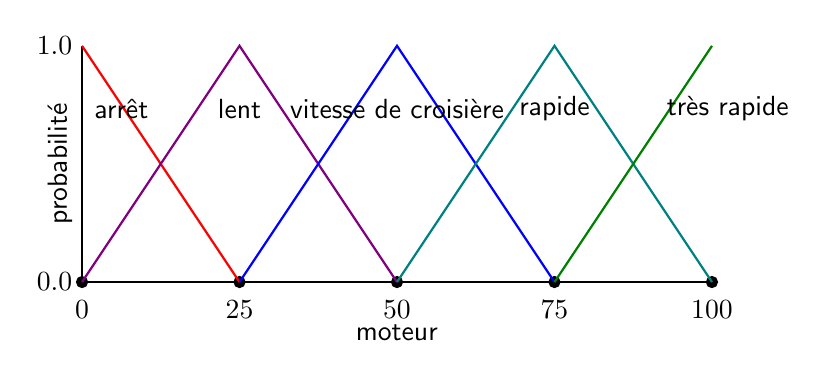
\begin{tikzpicture}
\draw (0,0) node[left] {\p{0.0}} -- node[sloped,above] {\textsf{probabilité}} (0,3) node[left] {\p{1.0}};
\draw (0,0) -- node[below,yshift=-12pt] {\textsf{moteur}} (8,0);
\foreach \n/\x in {0/0,25/2,50/4,75/6,100/8} {
  \draw[fill] (\x,0) circle [radius=2pt];
  \node at (\x,-10pt) { \p{\n} };
}
\draw[red,thick] (0,3) -- (2,0);
\draw[red!50!blue,thick] (0,0) -- (2,3) -- (4,0);
\draw[blue,thick] (2,0) -- (4,3) -- (6,0);
\draw[blue!50!green,thick] (4,0) -- (6,3) -- (8,0);
\draw[green!50!black,thick] (6,0) -- (8,3);
\node at (.5,2.2) {\textsf{arrêt}};
\node at (2,2.2) {\textsf{lent}};
\node at (4,2.2) {\textsf{vitesse de croisière}};
\node at (6,2.2) {\textsf{rapide}};
\node at (8.2,2.2) {\textsf{très rapide}};
\end{tikzpicture}
\caption{Déflouter pour obtenir un réglage robuste du moteur}\label{fig.defuzz}
\end{center}
\end{figure}

Supposons que la probabilité de la valeur de \p{cruise} soit calculée à $0,4$. Le triangle central de la Fig.~\ref{fig.defuzz} n'est alors plus pertinent car la probabilité ne peut jamais être supérieure à $0,4$, ce qui est représenté par un trapèze dans la Fig.~\ref{fig.trap}.

\begin{figure}
\begin{center}
% Areas defined by the certainties of the consequents
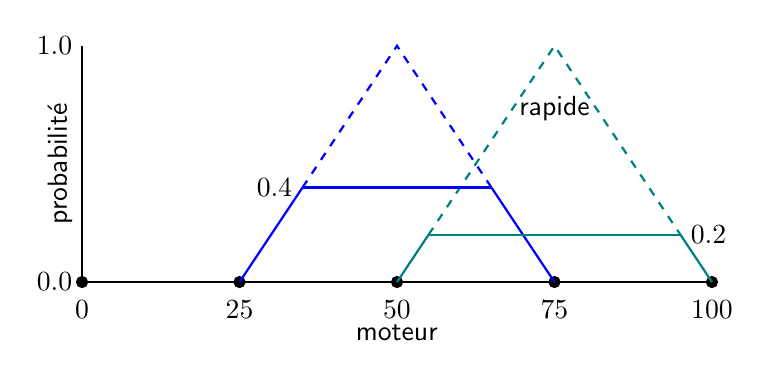
\begin{tikzpicture}
\draw (0,0) node[left] {\p{0.0}} -- node[sloped,above] {\textsf{probabilité}} (0,3) node[left] {\p{1.0}};
\draw (0,0) -- node[below,yshift=-12pt] {\textsf{moteur}} (8,0);
\foreach \n/\x in {0/0,25/2,50/4,75/6,100/8} {
  \draw[fill] (\x,0) circle [radius=2pt];
  \node at (\x,-10pt) { \p{\n} };
}
\draw[blue,thick] (2,0) -- (2.8,1.2);
\draw[blue,thick] (5.2,1.2) -- (6,0);
\draw[blue,thick,dashed] (2.8,1.2) -- (4,3) -- (5.2,1.2);
\draw[blue!50!green,thick] (4,0) -- (4.4,.6);
\draw[blue!50!green,thick] (7.6,.6) -- (8,0);
\draw[blue!50!green,thick,dashed] (4.4,.6) -- (6,3) -- (7.6,.6);
node at (4,2.2) {\textsf{cruise}};
\node at (6,2.2) {\textsf{rapide}};
\draw[blue,thick] (2.8,1.2) node[black,left] {\p{0.4}} -- (5.2,1.2);
\draw[blue!50!green,thick] (4.4,.6) -- (7.6,.6) node[black,right] {\p{0.2}};
\end{tikzpicture}
\caption{Domaines définis par les probabilités des valeurs}\label{fig.trap}
\end{center}
\end{figure}

Soit $w$ et $h$ la largeur et la hauteur d'un triangle. Alors l'aire d'un trapèze délimité par la droite de hauteur $h'$ est donnée par la formule:\footnote{La dérivation de la formule est donnée dans l'annexe~\ref{a.trap}.}
\begin{displaymath}
wh'\left(1-\frac{h'}{2h}\right)\,.
\end{displaymath}
Il est possible que plus d'une valeur ait des valeurs positives. La figure \ref{fig.trap} montre les trapèzes pour la valeur \p{vitesse de croisière} avec une probabilité de $0.4$ et la valeur \p{fast} avec une probabilité de $0.2$. Pour $w=50$, $h=1$, $h_{c}'=0.4$ (\p{cruise}), $h_{f}'=0.2$ (\p{fast}), les aires des trapèzes $a_c$ (\p{cruise}) et $a_f$ (\p{fast}) sont :

\begin{displaymath}
\spacearray
\begin{array}{l}
a_c = 50\times 0.4 \left(1 - \frac{0.4}{2}\right) = 16\\
a_f = 50\times 0.2 \left(1 - \frac{0.2}{2}\right) = 9\,.
\end{array}
\end{displaymath}
Pour obtenir une valeur précise, on calcule le \emph{centre de gravité}. Il s'agit de la somme des surfaces des trapèzes pondérée par la valeur au centre de la base de chaque trapèze divisée par la somme des surfaces :
\begin{displaymath}
\frac{16\times 50 + 9\times 75}{16+9}=59\,.
\end{displaymath}
La valeur est plus proche de la valeur associée à \p{vitesse de croisière} que de la valeur associée à \p{rapide}. Cela n'est pas surprenant puisque la probabilité de \p{vitesse de croisière} est plus grande que la probabilité de \p{rapide}.

\begin{framed}
\act{Logique floue}{fuzzy}
\begin{itemize}
\item Mettre en œuvre le contrôleur à logique floue pour un robot s'approchant d'un objet.
\item Définir les seuils appropriés pour le capteur de proximité et les valeurs appropriées pour le défloutage afin d'obtenir une vitesse de moteur précise.
\item Comparez les résultats avec l'algorithme de contrôle proportionnel que vous avez implémenté dans l'activité~\ref{act.proportional}.
\end{itemize}
\end{framed}

\section{Résumé}

Le contrôle par logique floue est une alternative aux algorithmes de contrôle mathématiques classiques décrits au Chap.~\ref{ch.control}. L'avantage de la commande par logique floue est qu'elle n'exige pas de spécifications mathématiques précises du comportement du robot, qui peuvent être difficiles à définir. Nous avons donné l'exemple des définitions floues de la vitesse ; d'autres exemples seraient la couleur (quand une nuance de rouge devient-elle orange ?) et la température (quand une pièce chaude devient-elle chaude ?). L'inconvénient est que le comportement de la commande à logique floue n'est pas aussi transparent que celui des algorithmes de commande classiques.

\section{Pour aller plus loin}

Les premiers travaux sur la logique floue ont été réalisés par Lotfi Zadeh \cite{zadeh}. Un ouvrage sur l'application de la logique floue au contrôle est \cite{passino}.  La logique floue est également utilisée dans le traitement des images \cite[Sect.~3.8]{GW}.
